\documentclass[a4paper,11pt]{article}
\usepackage[a4paper, left=1.5cm, right=1.5cm, top=2.0cm, bottom=3.5cm, headsep=1.2cm]{geometry}
\usepackage{polski}
\usepackage{amssymb}
\usepackage[utf8]{inputenc}
\prefixing
\usepackage{latexsym}
\usepackage{graphicx}
\author{Klaudia Balcer}
\title{Raport }
\frenchspacing
\begin{document}
\maketitle
\tableofcontents
\pagebreak


\section{model z interakcją a model bez interakcji}

\begin{tabular}{|c|c|c|c|c|c|}
model & untercept - pvalue & numeracy - pvalue & anxiety - pvalue & anxiety*numeracy - pvalue & AIC \\ \hline
z interakcją & 0.985 & 0.684 & 0.891 & 0.774 & 36.201 \\
bez interakcji  & 0.03623 & 0.01995 & 0.00396 & -- & 34.286 \\ 
\end{tabular}

Patrząc na wyniki test≤ów istotności w modelu z interakcją, dochodzimy do wniosków, że najprawdopodobniej, żadna ze zmiennych objaśniających nie ma istotnego wpływu na zmienną objaśnianą. Nie jest to dobry model. 

Patrząc na p-wartości w modelu bez interakcji, widzimy, że wszystkie uzyskane współczynniki są istotne - istanieje korelacja między obiema zmiennymi objaśniającymi a zmienną objaśnianą. Również AIC jest mniejsze w modelu bez interakcji, co również przemawia na jego korzyść. 


\section{modele z różnymi funckcjami linkującymi}

Dla wszystkich funckji linkujących krzywe ROC mają dość dużą całkę, co wskazuje, że mogą to dobre modele. Przyjrzyjmy się im bliżej, by móc przedstawić subtelniejsze różnice. 

Patrząc na testy istotności, widzimy, że model z użyciem funckji linkującej cauchit nie wskazuje na korelację zmiennych objaśniająych i objaśnianej. Ma on też wyraźnie większą wartość AIC. Użycie funkcji linkującej cauchit zdecydowanie nie jest optymalne. 

Wątpliwości może budzić również użycie funkcji cloglog. Zauważamy w tym modelu silną korelację między zmiennymi $X_{i}$ i $Y_{i}$. Testy jednak odrzucają istotność współczynnika $b_{0}$. Nie jest to najlepszy model, ale istotność współczynników dla zmiennych objaśniających jest cenna i skłania do dalszych badań nad danymi. 

Patrząc na współczynnik AIC jako najlepszą funkcję linkującą uznajemy probit. Wskazuje on na na istotność wszystkich współczynników modelu, co razem z dużym polem pod krzywą ROC zdecydowanie przemawia, za odpowiedniością tego modelu.

Podane wyżej wartości predykcyjnych prawdopodobieństw obliczyłam za pomocą funkcji predict z parametrem type = "response". Można to było również obliczyć \textit{ręcznie} ze wzoru:

$$ p_{i} = \frac{exp\{b_{0} + b_{1}X{1,i} + \ldots + b_{p-1}X_{p-1}\}}{1+exp\{b_{0} + b_{1}X{1,i} + \ldots + b_{p-1}X_{p-1}\}} $$

\begin{verbatim}
model <- glm(success~numeracy+anxiety, data=A, family=binomial(link = "cloglog"))
new <- data.frame(numeracy = c(10), anxiety = c(13))
predict.glm(model, new, type = "response")
b <- model$coefficients
exp(b[1]+b[2]*10+b[3]*13)/(1+exp(b[1]+b[2]*10+b[3]*13))
\end{verbatim}

To działanie dało identyczne wyniki (czego też się spodziewaliśmy), toteż nie odnotowywałam tego w sprawozdaniu dla poszczególnych grup. 

Do generowania krzywych ROC użyłam biblioteki ROCR.  

\subsection{logit}

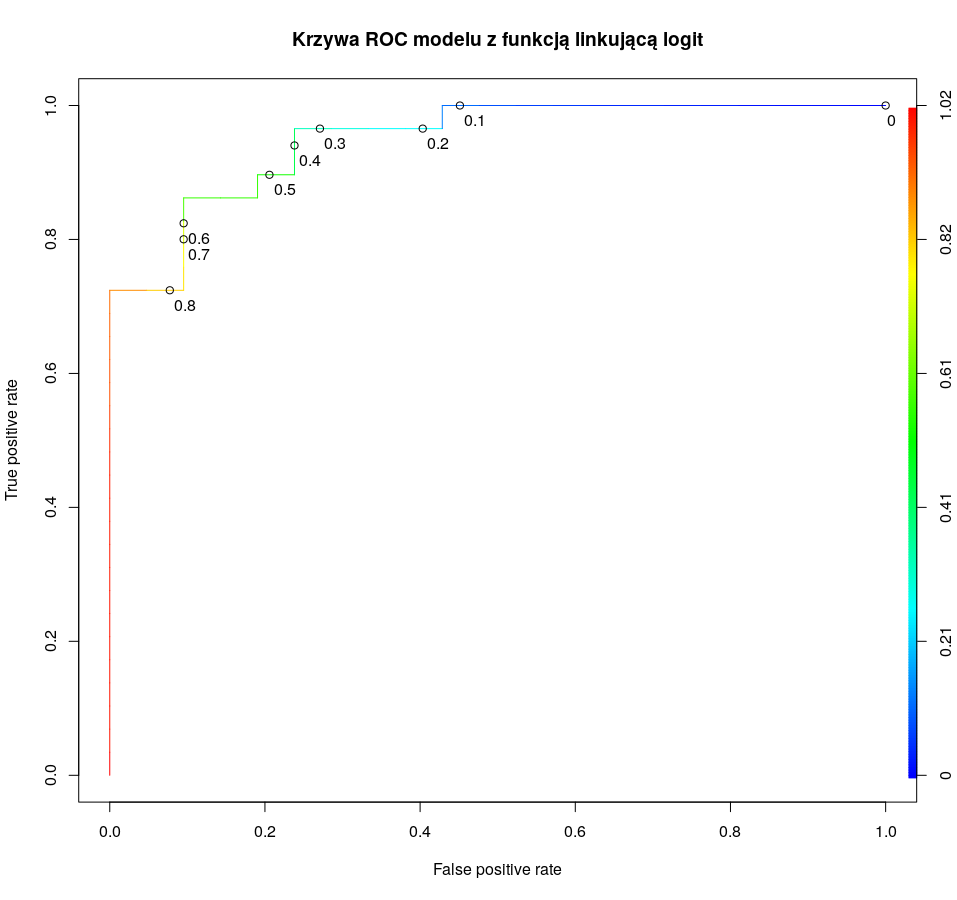
\includegraphics[scale=.25]{plot1.png} 

\begin{tabular}{|c|c|c|c|}
 & intercept & numeracy & anxiety \\ \hline
 wartość estymatora &  14.2386 &  0.5774  &   -1.3841   \\
 wartość statystyki & 2.094 & 2.327 &  -2.881 \\
 p-wartość &  0.03623 &   0.01995 &  0.00396  \\
 wynik tetstu istotności & + & + & ++ \\ \hline
\end{tabular}

AIC  =  34.286

$\widehat{P}(n  = 10, a = 13)$  = 0.8827987 
\subsection{probit}
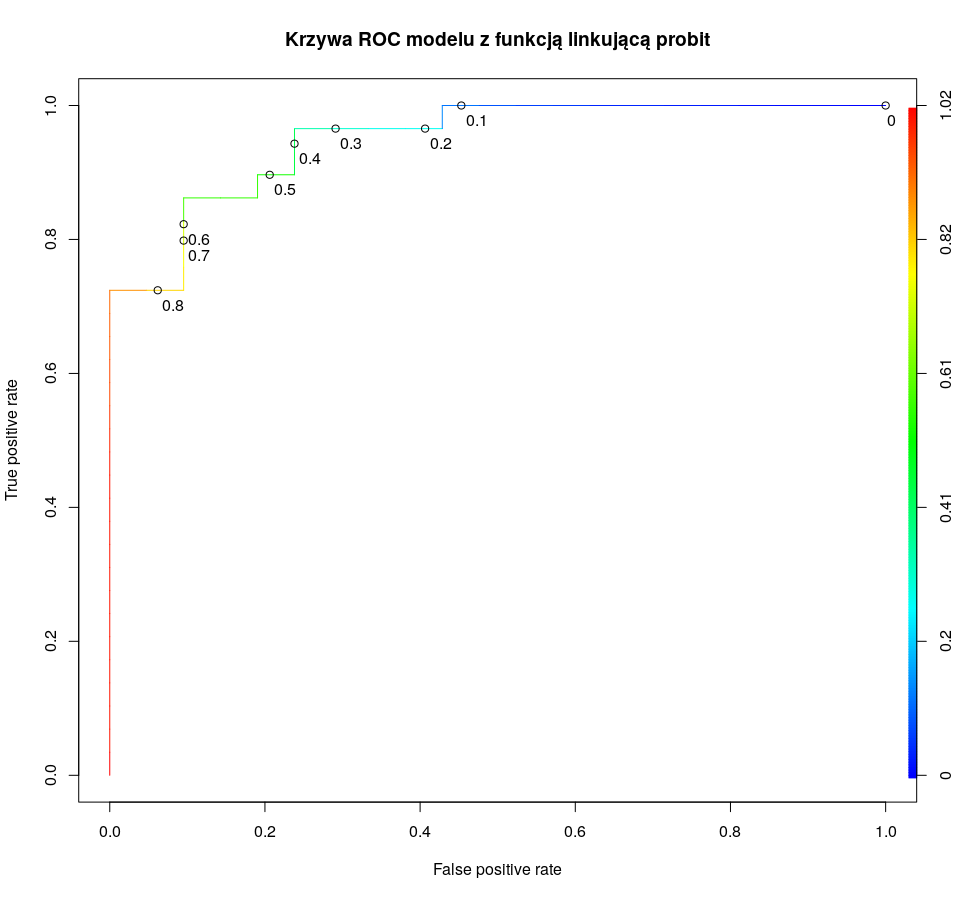
\includegraphics[scale=.25]{plot2.png}

\begin{tabular}{|c|c|c|c|}
 & intercept & numeracy & anxiety \\ \hline
 wartość estymatora &   8.2573  &   0.3371   & -0.8039  \\
 wartość statystyki &  2.247 &  2.464 &  -3.191 \\
 p-wartość &   0.02466 &  0.01374 &   0.00142 \\
 wynik tetstu istotności & + & + & ++ \\ \hline
\end{tabular}

AIC =  33.854

$\widehat{P}(n  = 10, a = 13)$  = 0.8806045 
 
\subsection{cauchit}
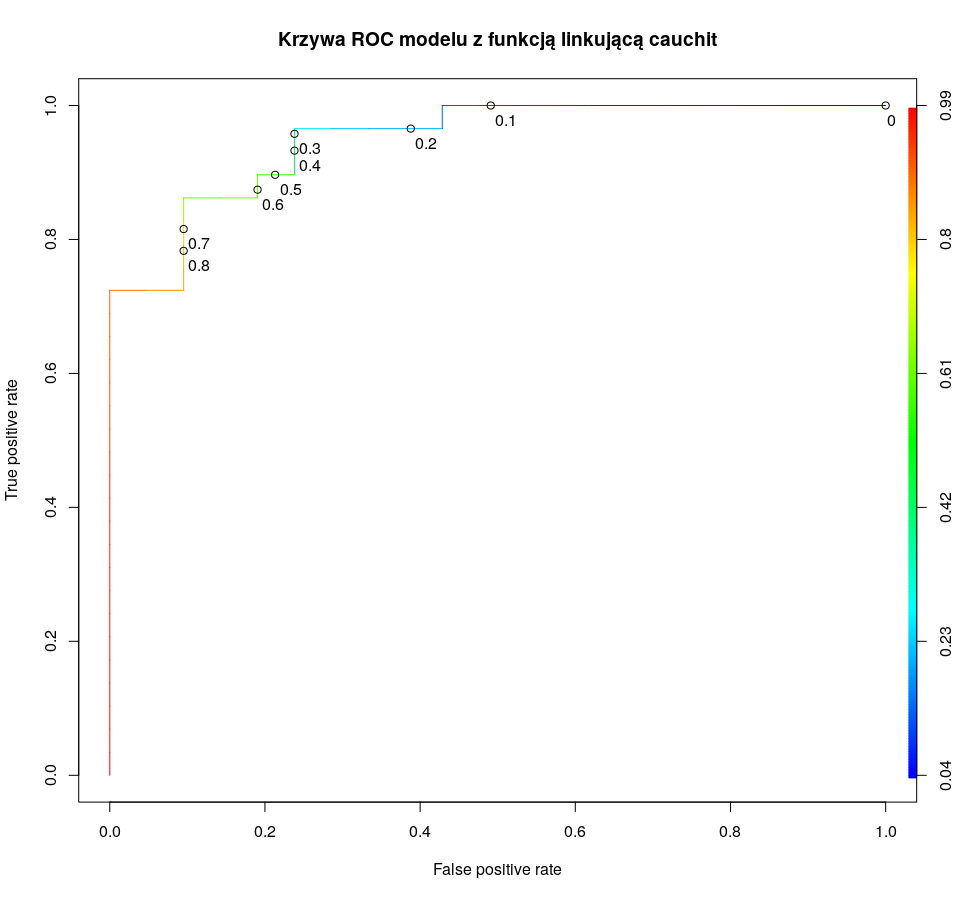
\includegraphics[scale=.25]{plot3.png} 

\begin{tabular}{|c|c|c|c|}
 & intercept & numeracy & anxiety \\ \hline
 wartość estymatora &  18.3830  & 0.7323  & -1.7741     \\
 wartość statystyki &   1.495  &  1.545 & -1.789 \\
 p-wartość &  0.1350   &  0.1224  &   0.0735\\
 wynik tetstu istotności & - & - & . \\ \hline
\end{tabular}

AIC = 37.115

$\widehat{P}(n  = 10, a = 13)$  = 0.8848509 

\subsection{cloglog}
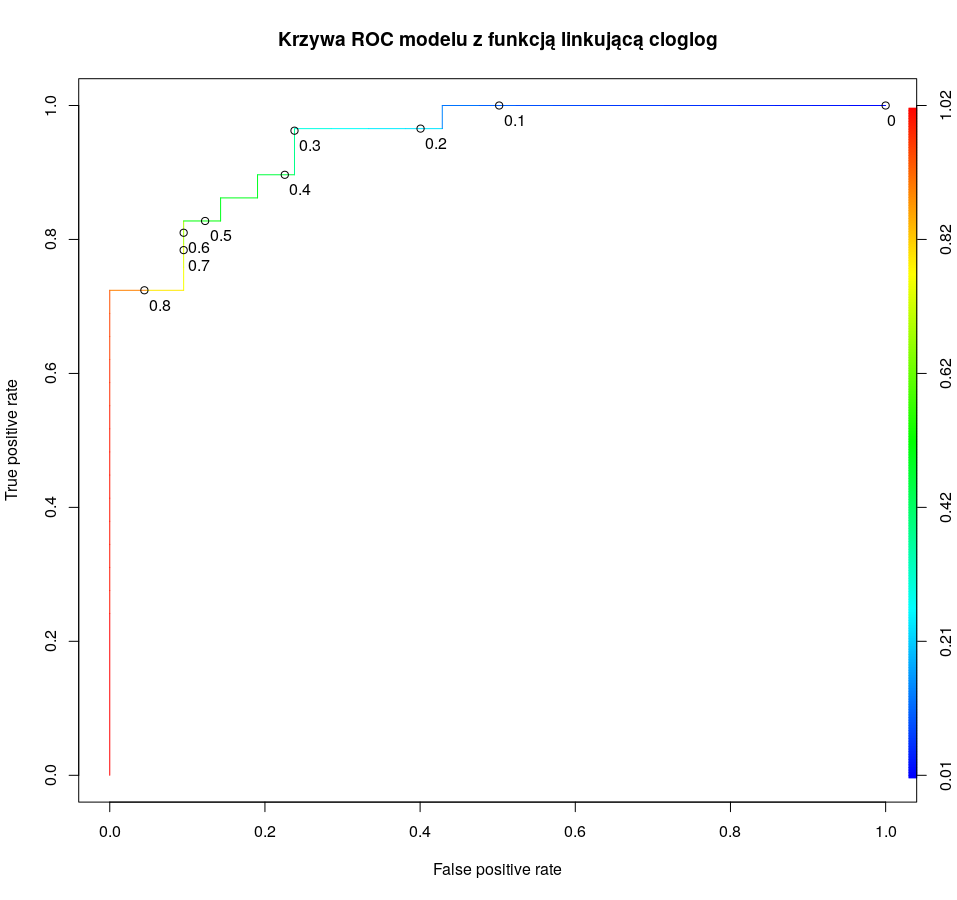
\includegraphics[scale=.25]{plot4.png} 

\begin{tabular}{|c|c|c|c|}
 & intercept & numeracy & anxiety \\ \hline
 wartość estymatora & 9.0006 & 0.4024 &  -0.9390   \\
 wartość statystyki &  1.935 & 2.644 &  -2.827  \\
 p-wartość &    0.05304  &  0.00819  &  0.00470    \\
 wynik tetstu istotności & . & ++ & ++ \\ \hline
\end{tabular}

AIC = 34

$\widehat{P}(n  = 10, a = 13)$  = 0.8963072



\end{document}